\chapter{Introduction (Français)}
\label{chap:intro-fr}

\margintoc

\selectlanguage{english}
\begin{kaobox}[backgroundcolor=Black!10!White,frametitlebackgroundcolor=Black!10!White]
  This \lcnamecref{chap:intro-fr} is an introduction intended for French-speaking readers.
  If your English is better than your French,
  you should instead read \cref{chap:intro-en}, its translation in English.
\end{kaobox}
\selectlanguage{french}

Cette thèse se situe dans le domaine de la \kl[type dépendant]{théorie des
types (dépendants)}, lui-même au croisement entre informatique et logique mathématique.
L’objectif principal est de participer aux fondements théoriques et pratiques des outils
que l’on appelle \kl{assistants à la preuve}, des logiciels qui, comme leur nom
l’indique, ont pour but d’assister des êtres humains dans la construction
et la vérification de preuves – au sens mathématique du terme. Il sera dans cette thèse
en particulier beaucoup question de l’assistant à la preuve \kl{Coq}, qui est celui
sur lequel mon travail s’est principalement concentré.

Pour replacer ce travail dans son contexte large, cette introduction commence par une histoire très parcellaire (et orientée) de la logique mathématique
(\cref{sec:logique-histoire}),
puis une présentation des assistants à la preuve,
notamment ceux qui, comme \kl{Coq}, se basent sur la théorie des types (\cref{sec:assistants-preuve}). Enfin la \cref{sec:cette-these} présente
mes contributions personnelles cette thèse.

\section{Une (très courte) histoire de la logique}
\label{sec:logique-histoire}

\subsection{Les syllogismes}
Dans la tradition occidentale, on peut faire remonter l’étude de
la logique à Aristote, dans son \textit{Organon}.
L’un des apports de ce travail est d’introduire les syllogismes.\sidenote{
  Le syllogisme le plus connu est probablement Barbara, dont un exemple est :
  \emph{tous les humains sont mortels ; Socrate est humain ; donc Socrate est mortel.}
}
Il s’agit de raisonnements dont la validité tient seulement au fait qu’ils
suivent une structure générale, et non à son contenu particulier.
Si un raisonnement est construit en assemblant ces syllogismes,
le raisonnement dans son entier doit nécessairement l’être également, puisque
chaque pas de raisonnement est valide.
L’idée importante ici est celle de décomposition en composantes élémentaires. À
partir d’un système de règles de raisonnement qu’on a identifiées comme valides 
\textit{a priori},\sidenote{
  Il peut s’agir de syllogismes, mais de bien d’autres systèmes… On en rencontra
  un certain nombre dans cette thèse !
}
on a un moyen de s’assurer de la validité de raisonnements potentiellement
très complexes.
Il suffit de vérifier qu’ils peuvent être décomposés à partir
des règles de base – et, bien entendu, que celles-ci soient correctes.

\subsection{Les débuts de la logique mathématique}
À la suite d’Aristote, les mathématicien·ne·s se sont emparé·e·s de la question
de la logique, en cherchant comment il était possible de fonder les mathématiques
rigoureusement. Bien qu’il s’agisse d’une question ancienne, de véritables
progrès concrets sur sa résolution ont commencé à voir le jour dans la deuxième
moitié du 19\textsuperscript{e} siècle, sur deux fronts principaux.

Le premier a consisté à se dégager du langage dit
naturel\sidenote{
  Par opposition aux langages formels qui apparaissent
  en mathématiques, informatique, etc.
}, inadapté pour la description formellement précise de la déduction, et à
concevoir à la place une nouvelle forme de langage spécifique qui puisse servir de
base à un système de raisonnement. Une étape importante
de cette ligne de recherche est
probablement \sidecite{Begriffsschrift}, qui introduit un certain nombre de
caractéristiques des langages dont il sera question dans la suite de cette thèse,
en particulier la notion de quantificateur.

Le second a pour but de montrer que les mathématiques dans leur entier peuvent
effectivement être reconstruites à partir de briques élémentaires. Une étape
importante ici a été la réduction de l’analyse à un petit nombre de propriétés
des nombres réels, puis les constructions de ces nombres réels à partir
de l’arithmétique, données quasiment simultanément par entre autres Dedekind
\sidecite{Dedekind1872} et \sidecite{Cantor1872}.
De son côté Peano \sidecite{Peano1889} propose
une axiomatisation des nombres entiers proche de celle encore utilisée aujourd’hui.
Enfin Cantor \sidecite{Cantor1883}
propose la théorie des ensembles comme un formalisme permettant
de décrire la totalité des objets mathématiques sous la forme d’ensemble
d’éléments.

\subsection{La crise des fondements}
Hélas, le système proposé dans \sidecite{Begriffsschrift}, fortement inspiré par
les travaux de Cantor, est inconsistant\sidenote{
  C'est-à-dire qu’il permet de prouver le faux, et donc qu’il ne peut pas servir
  de base valide pour la logique.
} !
Ce constat, dû à Russell \sidecite[][Nachwort p.~253]{Frege1903},
ouvre une période de crise, où la problématique de décrire un système qui permette
de fonder l’entièreté des mathématiques,
tout en évitant les inconsistances desquelles
le système de Frege et probablement ceux de Cantor étaient victimes.

Une première proposition de solution est avancée par Whitehead et Russell
avec \sidecite{Whitehead1913}, un énorme travail qui non seulement propose un système
logique qui évite les paradoxes conduisant à l’inconsistance de
\sidecite{Begriffsschrift}, mais de plus réalise dans ce système une quantité importante
de mathématiques, en particulier une construction des entiers, de l’arithmétique et
finalement des nombres réels.

En parallèle, dans la continuité des travaux de Cantor,
Zermelo \sidecite{Zermelo1908} et
d’autres travaillent à fournir une description formelle de la théorie des ensemble
qui soit consistante. Ceci aboutit à ce qu’on appelle de nos jours la
théorie des ensembles de Zermelo-Fraenkel (ZF, ou ZFC quand on y ajoute l’axiome
du choix), qui semble également à même de fournir une base solide pour les
mathématiques.

\paragraph{L’incomplétude.}
Un deuxième coup vient cependant frapper la recherche d’un système adéquat pour
servir de fondation aux mathématiques : le théorème d’incomplétude de Gödel
\sidecite{Goedel1931}. Celui-ci affirme que tout système formel
dans lequel on peut construire des nombres entiers comme de Peano – donc
\textit{a fortiori} tout système suffisamment riche pour faire des mathématiques –
ne peut pas démontrer sa propre consistance. Ainsi, il n’existe pas de
système sur lequel on puisse fonder les mathématiques en ayant la certitude
formelle que ce système est adéquat : puisqu’on ne peut prouver la consistance du
système dans lui-même, il pourrait finalement s’avérer inconsistant, ruinant les
efforts fournis.

Une conséquence de ce théorème est qu’un système suffisamment riche
pour faire des mathématiques est nécessairement incomplet.\sidenote{
  Cela signifie qu’il
  existe des énoncés indépendants, à savoir des assertions qu’on ne peut
  ni démontrer, ni réfuter – c’est-à-dire montrer la négation. La consistance du
  système considéré en est un exemple.
}
Ainsi, dans la suite il ne sera jamais question de vérité absolue –
ce qui n’aurait de sens que dans un système complet
où tout énoncé est vrai ou faux –, mais
uniquement de prouvabilité \emph{dans un système donné}.

\subsection{Une première conclusion}
Malgré les difficultés mises au jour au début du 20\textsuperscript{e}
siècle, la communauté mathématique est globalement
satisfaite de la situation : ZFC fournit un système raisonnable sur
lequel baser en principe toutes les mathématiques, et même si peu de
personnes se risquent à tenter, dans la veine de \cite{Whitehead1913},
d’effectivement écrire leurs mathématiques à ce niveau de précision,
elle est globalement convaincue que ce serait en théorie
possible, et cela suffit amplement à la plupart.

De plus, le développement et la vérification humaine de mathématiques véritablement
formalisées semble essentiellement impossible et inutile.
D’un côté, cela demanderait un effort considérable,
tant de la part de l’autrice que de celle de la lectrice, tout en étant
extrêmement laborieux et désagréable.
Dans le même temps, cela ne permettrait pas de réduire de manière importante
les risques d’erreurs, puisqu’il est
humainement très difficile de détecter une petite erreur au milieu de centaines de pages de raisonnement.
Enfin, décrire les mathématiques à ce niveau obscurcirait
considérablement les intuitions mathématiques importantes,
rendant la communication stérile.

\section{Les ordinateurs entrent en scène}
\label{sec:assistants-preuve}

Un nouvel élément vient cependant changer fondamentalement cette situation :
l’avènement des ordinateurs.

\subsection{Pourquoi les ordinateurs ?}

Les ordinateurs excellent là où les humains pêchent : leur spécialité est de traiter
d’immenses volumes d’information très précise, exactement le type
de besoins que soulève la manipulation de preuves formelles. C’est pourquoi, dès
le début des années 70\sidenote{
  Avec des systèmes comme Automath \cite{DeBruijn1970}, Mizar \cite{Rudnicki1992}…}
ont commencé à apparaître ce que l’on appelle \intro{assistants à la
preuve}, des outils informatiques servant à écrire, vérifier et communiquer des
preuves.
Via la formalisation de ces preuves et la vérification par l’ordinateur qu’elles
suivent bien les règles du système logique sous-jacent, les assistants à la preuve
donnent accès à une fiabilité bien plus important que celle des preuves
traditionnelles. Des mathématiciens reconnus comme
Voevodsky~\sidecite{Voevodsky2010},
Hales~\sidecite[][Preface, p. xi]{Hales2012},
ou Scholze~\sidecite{Scholze2021}
se sont déjà emparés des assistants à la preuve,
notamment dans le but de lever les incertitudes
sur la solidité de leur propre travail.

Mais le terme d’\emph{assistant} à la preuve n’a pas été choisi par hasard : au-delà
de la simple vérification, les assistants à la preuve ouvrent la porte à un large
éventail d’outils mis à la disposition de la programmeuse, souvent de façon
interactive. La preuve est ainsi construite comme le produit d’un échange entre 
la programmeuse et l’outil, plutôt que fournie d’un seul bloc.
Il peut s’agir de simples
facilités, comme la possibilité de pouvoir visualiser la structure des
preuves, de suivre l’utilisation des hypothèses…
Mais l’informatique rend surtout possible l’automatisation de pans entiers
de l’écriture de preuves,
par exemple via l’utilisation d’un langage de tactique \sidecite{Delahaye2000}
qui permettent de programmer la manière dont les preuves sont
générées, voire en utilisant directement la recherche en preuve automatique
\sidecite{Boehme2010,Ekici2017}.
\textit{In fine}, cette automatisation permet généralement d’écrire
les preuves à haut niveau, en laissant à l’assistant à la preuve le soin
de construire une preuve formelle.
Un autre axe important, bien qu’encore relativement peu développé, concerne
les interactions entres les outils informatiques dédiés au calcul mathématique
(systèmes de calcul formel, analyse numérique) et les assistants à la
preuve sont une piste très prometteuse.

Enfin, si l’utilisation de programmes de toutes sortes permet de grandement augmenter
les possibilités offertes par les assistants à la preuve,
la présence au même endroit – l’ordinateur –
de preuves et de programmes est également parfaite pour… la preuve de programmes.
Ils offrent en effet un cadre naturel dans lequel décrire au même endroit
le code source d’un programme, sa spécification et la preuve formelle que le
programme s’exécute correctement,
remplissant sa spécification sans rencontrer de bug.

\subsection{Logique, programmation et théorie des types}

Pour fonctionner, les assistants à la preuve ont besoin d’une
description formelle des "règles du jeu" mathématiques qu’ils sont censés imposer.
En clair, ils demandent une étude renouvelée de la logique, mais dans le but
pratique de construire des outils à la fois fonctionnels,
puissants et faciles à utiliser.
Il existe plusieurs familles d’assistants à la preuve, basées sur des fondements
logique relativement différents. La famille qui m’intéresse dans cette thèse, est
celle à laquelle appartient \kl{Coq}, celle basée sur la
\kl{correspondance de Curry-Howard} et la \kl[type dépendant]{théorie des types dépendants}.

Si on compare un programme informatique à un texte dans une langue naturelle,
les types sont une sorte d’équivalent des catégories grammaticales.
Contrairement aux langues naturelles, cependant, ces règles de typage sont conçues
en même temps que le langage de programmation, en général
de telle sorte à refléter des propriétés
des objets manipulés par le programme. Cela permet en premier lieu de
détecter des erreurs manifestes.
Par exemple, si une procédure attendant un objet de type "image" est
appliquée à un objet de type "chaîne de caractères", une erreur pourra être rapportée
à la programmeuse.\sidenote{
  Un slogan dû à Milner~\sidecite[5em]{Milner1978} est que
  « Les programmes bien typés ne peuvent pas  mal s’exécuter. »
}
Mais les utilisations des types sont très versatiles, et leurs capacités à encoder
des propriétés des programmes sous-jacents peuvent servir à la compilation, la
documentation, etc.

\begin{marginfigure}[2em]

  % \begin{mathpar}
  %   \inferrule{ \Gamma, A \vdash B}{\Gamma \vdash A \Rightarrow B} \and
  %   \inferrule{\Gamma \vdash A \Rightarrow B \\ \Gamma \vdash A}{\Gamma \vdash B} \and
  %   \inferrule{\Gamma, x : A \vdash t : B}{\Gamma \vdash \lambda x : A . t : A \to B} \and
  %   \inferrule{\Gamma \vdash f : A \to B \\ \Gamma \vdash u : A}{\Gamma \vdash f~u : B}

  % \end{mathpar}

  % \caption{Règles d’inférence pour l’implication et de typage des fonctions}

  \begin{mathpar}
    \inferrule*{A \\ B}{A \wedge B} \and
    \inferrule*{A \wedge B}{A} \and
    \inferrule*{A \wedge B}{B} \\
    \inferrule*{a : A \\ b : B}{(a,b) : A \times B} \\
    \inferrule*{p : A \times B}{p.1 : A} \and
    \inferrule*{p : A \times B}{p.2 : B}
  \end{mathpar}
  
  \caption{Règles d’inférence pour la conjonction et de typage pour les paires}
  \label{fig:curry-howard-exemple}
\end{marginfigure}

Plutôt qu’un théorème précis, la \intro{correspondance de Curry-Howard} est une
idée très générale,
selon lequel il existe une ressemblance forte entre d’un côté le monde de la
logique et des preuves, et de l’autre celui des programmes et de leurs types.
Un exemple valant mieux qu’un discours abstrait, on peut voir la correspondance à l’œuvre dans la \cref{fig:curry-howard-exemple}, sous la forme de règles d’inférence
ou de typage : chaque bloc présente une règle, avec au-dessus de la barre les
hypothèses, et en dessous la conclusion.
Les trois premières règles gouvernent la conjonction logique $\wedge$.
La première signifie que pour déduire la proposition $A \wedge B$,
il suffit de déduire $A$ et $B$ individuellement.
À l’inverse si a comme hypothèse $A \wedge B$, alors on peut déduire $A$ et $B$
individuellement.
Les trois dernières règles gouvernent le typage du type des paires $A \times B$.
Une paire $(a,b)$ a le type $A \times B$ si $a$ est de type $A$ et $b$
est de type $B$.
À l’inverse si $p$ est de type $A \times B$, alors sa première projection $p.1$
est de type $A$ et sa seconde projection $p.2$ est de type $B$.
Si on efface les termes\sidenote{
  Dans ce contexte, on parle souvent de \emph{termes} plutôt que de programmes,
  mais les deux sont synonymes.
} des règles du bas, on obtient \emph{exactement} les règles du haut !

Ceci s’étend bien au-delà du cas de la conjonction,
en une correspondance générale entre d’une part les énoncés de la logique et les types des langages de programmation , et d’autre part les preuves d’un énoncé et les programmes ayant le type correspondant\sidenote{
  Le slogan en anglais est \textit{propositions as types, proofs as programs}.}.
Au-delà de la simple analogie entre formalismes d’origines différentes, cette correspondance est un outil puissant pour faire dialoguer deux mondes.
En particulier, elle permet de relier deux problèmes \textit{a priori} éloignés :
la vérification de la correction d’une preuve et l’analyse du type d’un terme.

La \kl{correspondance de Curry-Howard} est donc idéale pour servir de fondements aux
assistants à la preuve, puisqu’elle permet de voir un système
comme une logique, tout en autorisant l’utilisation d’idées venant de
la large littérature sur les langages de programmation, notamment
la théorie et l’implémentation des systèmes de types.
Dans ce cadre, les \intro[type dépendant]{systèmes de types dépendants} sont une famille dont
la caractéristique principale, comme leur nom l’indique, est d’autoriser les
types à dépendre de termes. L’exemple archétypique du point de vue de la 
programmation est le type
$\Vect A n$ des listes contenant exactement $n$ éléments
de type $A$ – avec $n$ un entier.
Du point de vue de la logique, cette
dépendance correspond aux quantificateurs, nécessaires pour exprimer des
propriétés universelles – pour tout entier $n$, la propriété $P(n)$ est
vérifiée — et existentielles – il existe un entier $n$ tel que $P(n)$ tient –,
sans lesquelles il est tout bonnement impossible d’exprimer la plupart des
mathématiques. En revanche les systèmes à types dépendants, eux, sont suffisamment
riches et puissant pour espérer y développer la plupart des mathématiques.

\section{Coq et son noyau}
\label{sec:intro-coq}

Intéressons-nous maintenant un peu plus précisément à l’assistant à la
preuve dont il sera le plus question dans cette thèse : \intro{Coq}.

\subsection{La clé de voûte du système}

\begin{figure}[h]

  \centering
  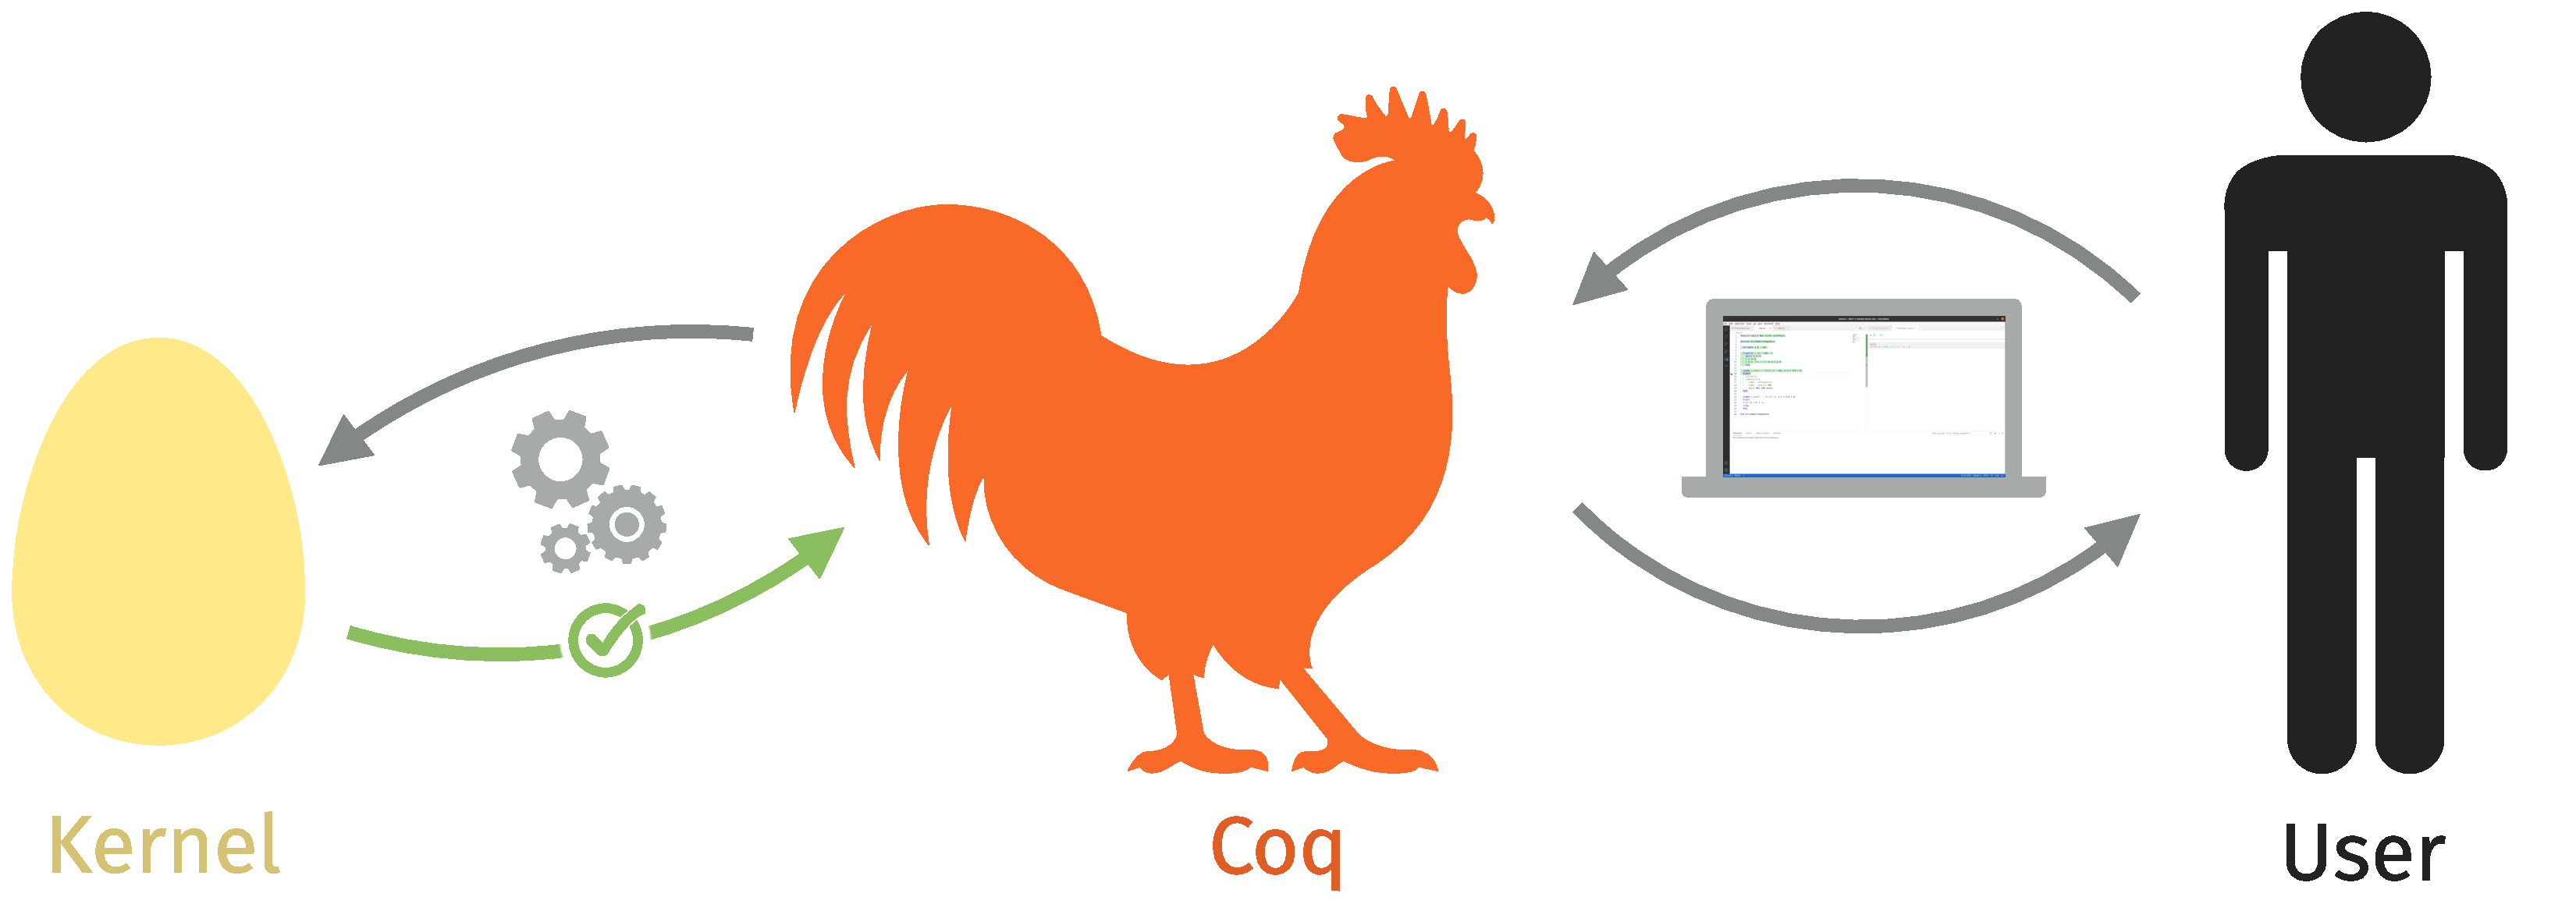
\includegraphics{./figures/coq-kernel-fr.pdf}

  \caption{Le fonctionnement schématique de Coq}
  \label{fig-coq}
\end{figure}

Coq est basé sur la \kl{correspondance de Curry-Howard} : les preuves sont vues comme des programmes dans un langage appelé \intro{Gallina},
et leur vérification est effectuée par un algorithme proche
de ceux utilisés pour les types des langages conventionnels.
Cependant, si dans les premières versions des années 80 \kl{Coq} ressemblait à un langage de programmation un peu étrange, ce n’est actuellement plus du tout le cas.
La raison, comme on l’a expliqué plus haut, est que \kl{Coq} est un \emph{assistant} à la preuve.
C’est pourquoi la majeure partie de \kl{Coq} dans ses versions actuelles a pour but d’aider l’utilisatrice à générer une preuve correcte sans avoir à l’écrire directement.
Ce fonctionnement est illustré en \cref{fig-coq} : l’utilisatrice échange interactivement avec \kl{Coq}, qui utilise cette interaction pour générer un terme de preuve. Celui-ci est ensuite envoyé à une partie bien spécifique du système, appelée \intro{noyau}.
C’est lui qui implémente l’algorithme de vérification de type, et s’assure ainsi de la correction des termes de preuve construits interactivement.
Le \kl{noyau} est donc l’élément crucial du système, car c’est lui – et lui seul – qui est responsable en dernier recours de la validation des preuves.


Cette architecture, qui isole clairement la partie critique du système
est appelée \intro{critère de de Bruijn} \sidecite{Barendregt2001}, en 
hommage à l’un des pionniers des assistants à la preuve.
% Elle a permis de mener à bien des projets de grande ampleur, parmi lesquels CompCert \sidecite{Kaestner2017} – un compilateur optimisant pour le langage C entièrement prouvé correct –, ou les preuves du théorème des quatre couleurs \sidecite{Gonthier2007} et du théorème de l’ordre impair \sidecite{Gonthier2013}, deux théorèmes importants et difficiles respectivement de la théorie des graphes et des groupes.
Cependant, si le reste de l’écosystème s’est beaucoup plus développé que le \kl{noyau} depuis les débuts, celui-ci a également évolué, en se complexifiant graduellement.
Et comme tout développement logiciel, il n’est pas à l’abri de bugs\sidenote{De l’ordre d'un bug détecté par an, une liste est maintenue à l’adresse suivante : \url{https://github.com/coq/coq/blob/master/dev/doc/critical-bugs}.}.
Ceux-ci sont en général difficilement exploitables par une utilisatrice de \kl{Coq}, encore plus sans s’en rendre compte.
Néanmoins, ils existent, et la tendance à la complexification du \kl{noyau} ne risque pas de s’arrêter de si tôt.

\subsection{MetaCoq, une formalisation par Coq, pour Coq}
\label{sec:intro-metacoq}


Si on veut garantir un niveau de fiabilité le plus élevé possible, il faut donc de nouvelles idées.
Le projet \intro{MetaCoq}, a pour but de répondre à cette problématique.
L’idée est simple : il s’agit d’utiliser \kl{Coq} lui-même pour certifier la correction de son \kl{noyau}.

Plus précisément, la première étape est de décrire à haut niveau le système de type sur lequel est basé le \kl{noyau}, puis de démontrer ses propriétés théoriques.
% , comme la confluence de la réduction, la préservation du typage par cette même réduction, etc.
Une fois ces propriétés établies, la deuxième étape consiste à programmer un algorithme de vérification de type ressemblant au maximum à celui du \kl{noyau}, directement en \kl{Gallina},\sidenote{
  En effet, grâce à la \kl{correspondance de Curry-Howard}, \kl{Gallina} est certes un langage pour décrire des preuves, mais aussi un véritable langage de programmation fonctionnel !}
tout en démontrant qu’il est bien correct\sidenote{
  Si l’algorithme prétend qu’un terme est bien typé, alors c’est bien le cas.}
et complet\sidenote{
  L’algorithme répond bien affirmativement sur tous les termes bien typés.}.
Enfin, une troisième étape extrait de ce programme \kl{Gallina} certifié
un programme efficace qui puisse être utilisé en lieu et place du \kl{noyau} actuel.
Cette extraction est elle-même complexe, car pour obtenir ce programme efficace il
faut effacer le contenu lié à la preuve de correction
pour ne garder que le contenu algorithmiquement intéressant.
C’est pourquoi là encore on prouve que l’extraction est correcte\sidenote{
  C'est-à-dire qu’elle préserve la sémantique des programmes.},
à nouveau en la programmant en \kl{Gallina}.

\subsection{Vérification et inférence}

Pour prouver la complétude de l’algorithme de typage, il est très utile de
passer par une spécification intermédiaire plus structurée que la description
théorique du système de type utilisée dans la première étape.
En particulier, il est important de séparer deux problèmes proches, mais
différents :
d'une part, la vérification, où on cherche à \emph{vérifier}
qu’un terme a bien un type
donné ; de l’autre, l’inférence, où on cherche à \emph{trouver}
un type pour un terme, s'il existe.
L’algorithme de typage du \kl{noyau} de \kl{Coq} est bidirectionnel,
c'est-à-dire qu’il alterne en permanence entre ces deux problèmes
lorsqu’il vérifie qu’un terme est bien typé.
% Par exemple, dans le cas d’une application $f~u$, il commence par inférer un type pour $f$, vérifie qu’il s’agit d’un type produit $\P x : A . B$ (une généralisation du type fonctionnel $A \to B$), puis vérifie que $u$ a le type $A$.
Décrire formellement cette structure bidirectionnelle plus proche de l’algorithme
permet de bien diviser les difficultés entre d’un côté
son équivalence avec la présentation
originale, et de l’autre la partie purement liée aux questions d’implémentation.

Dans le cadre spécifique des types dépendants, bien que présent depuis l’origine dans les algorithmes de vérification de type \sidecite{Huet1989},
le typage bidirectionnel a été étonnamment peu étudié. En particulier, une preuve
de l’équivalence entre cette présentation et celle utilisée de manière standard
dans la littérature manquait !
Pourtant, cette approche présente également
des avantages théoriques : elle permet,
par sa structure plus contrainte que la présentation standars,
d’obtenir des propriétés difficiles à démontrer dans ce cadre standard.

\subsection{Un peu de flexibilité dans un monde désespérément statique}
\label{sec:intro-graduel}

Comme le cas de \kl{MetaCoq} l’illustre, \kl{Coq} peut être utilisé comme un véritable langage
de programmation. Mieux : son système de type, grâce à son extrême expressivité, 
permet d’exprimer des propriétés très complexes des programmes, et de vérifier
avant même d’exécuter les programmes que celles-ci sont bien respectées par le code.
Cependant, cette impossibilité d’écrire du code imparfait peut aussi se retourner contre l’utilisatrice, en complexifiant la phase de développement.
En effet, personne n’écrit du code parfait au premier essai. Les garanties très
fortes sur le code une fois finalisé compliquent donc 
fortement la phase de développement.
Une solution pour faciliter cette phase de développement
est de s’inspirer d’une proposition issue de la théorie des langages de
programmation : le \kl{typage graduel}. Ici encore, la \kl{correspondance de Curry-Howard}
est à l’œuvre, puisqu’on adapte des concepts venant du monde de la programmation
au cadre de la logique.

Il existe deux grandes approches de la vérification du type des programmes.
Dans l’approche statique\sidenote{Qui est celle sur laquelle est basée \kl{Coq}.},
les types sont vérifiés en amont de l’exécution, alors que dans l’approche dynamique le bon typage des opérations est vérifié à la volée lors de cette même exécution.
La discipline dynamique est plus flexible, parce qu’elle permet de vérifier exactement ce qui est nécessaire à la bonne exécution d’un programme.
À l’inverse, la rigidité du typage statique permet de détecter des erreurs plus tôt dans le développement, et impose des invariants utiles pour optimiser la compilation ou l’exécution.
Pourquoi choisir ? Le programme de recherche du \intro{typage graduel} \sidecite{Siek2015} vise à dépasser ce dilemme, en intégrant dans un même langage disciplines statiques et dynamiques.
L’idée est d’avoir une première passe de vérification avant l’exécution, comme en typage statique, tout en laissant la possibilité de déférer des vérifications de type à l’exécution, comme en typage dynamique.
On a alors accès à tout un spectre de possibilités, d’une discipline totalement statique à une discipline totalement dynamique,
en pouvant choisir finement quelles parties d’un programme on veut vérifier à quel moment. En particulier, on peut faire évoluer la discipline au fur et à mesure d’un développement logiciel, pour bénéficier de la flexibilité du typage dynamique dans les phases précoces et des garanties du typage statique par la suite.

\section{Et cette thèse, alors ?}
\label{sec:cette-these}

Mon travail de doctorat lui-même
est centré principalement autour du typage bidirectionnel, sous
trois aspects, correspondant aux trois parties de cette thèse.

\subsection{Théorie du typage bidirectionnel}

La première partie (\nameref{part:bidir}) répare (une partie du) manque d'étude
théorique dans la littérature du typage bidirectionnel pour les types dépendant. Elle contient en particulier la
preuve de l’équivalence entre la présentation standard de la littérature et celle
bidirectionnelle.
Le \cref{chap:bidir-ccw} présente les idées générales qui guident ce travail
dans un cadre relativement simple, afin de faciliter leur exposition. 
Le \cref{chap:bidir-cic} montre comment étendre ces idées à un
cadre plus réaliste, proche de la théorie des types utilisée en pratique dans \kl{Coq}.
Enfin le \cref{chap:bidir-conv} traite du statut particulier de la
conversion\sidenote{Cette notion cruciale permet d’intégrer dans la
  théorie des types dépendants l’idée de calcul des programmes.}
et des liens du typage bidirectionnel avec certains travaux récents
à ce propos.

\subsection{Typage bidirectionnel dans MetaCoq}

La seconde partie de cette thèse (\nameref{part:metacoq})
concerne le projet \kl{MetaCoq}
et en particulier sur la formalisation, en \kl{Coq}, des idées présentées dans la
première partie. Le \cref{chap:metacoq-general} donne une présentation générale du
projet, tandis que le \cref{chap:kernel-correctness} se concentre spécifiquement
sur la preuve que le \kl{noyau} implémenté par \kl{MetaCoq} respecte sa spécification.

\subsection{Élaboration bidirectionnelle pour le typage graduel}

Enfin la troisième et dernière partie (\nameref{part:gradual})
présente mon travail
dans le domaine des \kl{types graduels}. Les types dépendants formant déjà des systèmes
complexes, l’adaptation de ceux-ci à l’approche graduelle est particulièrement
délicate. Un résumé des possibilités et problématiques associées est présentée
en \cref{chap:gradual-dependent}.
Un point intéressant est que la présentation habituelle
des types dépendants est inadaptée,
car elle est trop flexible. La structure additionnelle apportée
par le typage bidirectionnel est donc encore une fois cruciale.
De plus, celle-ci s’est avérée très agréable pour présenter
l’élaboration de termes depuis un langage source dans un langage cible, une
caractéristique importante des \kl[graduel]{langages graduels}.
L’utilisation d’une élaboration bidirectionnelle, et les propriétés qu’elle
permet d’obtenir, sont décrites en \cref{chap:bidir-gradual-elab}.

\subsection{Contributions personnelles}

Mon travail de doctorat a débuté avec l’étude des \kl{types dépendants} \kl{graduels}.
J’ai contribué avec Kenji Maillard, Nicolas Tabareau et Éric Tanter à
\sidecite{LennonBertrand2020}, où nous étudions une extension graduelle
pour le Calcul des Constructions Inductives. Mon travail technique s’est
majoritairement concentré sur le contenu correspondent au \cref{chap:bidir-gradual-elab}.
Le \cref{chap:gradual-dependent} est également tiré de cette publication.
Un second manuscrit avec les mêmes auteurs dans la continuité de
\cite{LennonBertrand2020} est actuellement en phase de relecture, mais il
ne fait pas appel directement au typage graduel, c’est pourquoi il n’en
sera pas question dans cette thèse.

Ce travail ayant montré la nécessité d’un système de types bidirectionnel
et le manque de résultats précis sur le sujet, je l’ai
étudié plus en détail, à la fois sur papier et par le biais d’une
formalisation se basant sur \kl{MetaCoq},
ce qui a donné lieu à une seconde publication
\sidecite{LennonBertrand2021}, et correspond aux
\cref{chap:bidir-ccw,chap:bidir-cic}, et à une partie du
\cref{chap:kernel-correctness}.

J’ai ensuite travaillé à intégrer cette formalisation à
\kl{MetaCoq}, et à l’utiliser afin de montrer la complétude du \kl{noyau}
qui y est implémenté. Ceci correspond au reste du \cref{chap:kernel-correctness}.
Au-delà de cette contribution principale,
j’ai également participé à ce projet sur d’autres points plus mineurs.
Cette partie de mon travail de thèse n’a pas encore été publié, mais nous y
travaillons actuellement avec les autres contributeurs de \kl{MetaCoq}.

Enfin le \cref{chap:bidir-conv} correspond à un travail que j’ai entamé dans
le but d’étendre \kl{MetaCoq}, mais qui n’a pas encore atteint le stade de la
publication.